%% ------------------------------------------------------------------------- %%
\chapter{Fundamentação Teórica}

\noindent O sistema ``\acrshort{uft} Serviços'' foi desenvolvido para atender a demanda da Direção e Prefeitura do Campus Universitário de Palmas da \acrshort{uft}, quanto à implantação de um sistema de abertura e acompanhamento de chamados para manutenção de equipamentos, através da utilização de dispositivos móveis com a plataforma \textit{Android} \cite{android} e aplicação \textit{web}, utilizando a tecnologia \gls{jsf} \cite{jsf} em conjunto com a biblioteca de componentes \textit{Primefaces} \cite{primefaces}.

Diante dessa necessidade observou-se a oportunidade da utilização da ferramenta de gerenciamento de serviços de \acrshort{ti}, o \acrshort{itil} v3, devido o fato deste possuir uma ampla documentação que fornece um conjunto de boas práticas para o gerenciamento de serviços de \acrshort{ti} em suas diversas etapas de implantação  por meio dos conceitos de estratégia, planejamento, transição, operação e continuidade do serviço \cite{servicestrategy, introductoryoverviewofitil}.

\section{Biblioteca \acrshort{itil}}

\noindent Após uma crescente demanda do governo do Reino Unido em gerenciar os serviços de \acrshort{ti} de forma eficiente, foi criado pela \gls{ogc} o \acrshort{itil} com o objetivo inicial de atender às necessidades das organizações públicas do governo inglês no gerenciamento dos serviços de \acrshort{ti}, de forma organizada \cite{itilservicemanagement}.
Em uma definição geral, \acrshort{itil} é um \textit{framework} que contém boas práticas para a gestão de serviços de \acrshort{ti} \cite{abreu2012implantando, servicestrategy, introductoryoverviewofitil}.


O \textit{framework} \acrshort{itil} é uma ferramenta que contém um conjunto de recomendações voltadas para \gls{itsm} que tem como propósito disponibilizar aos prestadores de serviços de \acrshort{ti} um guia detalhado sobre  como gerenciar seus serviços com qualidade \cite{servicestrategy}. As especificações deste \textit{framework} formam um resultado de anos de informações obtidas pela observação do trabalho de profissionais de \acrshort{ti} e processamento de dados ao redor do mundo, e por conta de sua amplitude de informações, tornou-se referência mundial como conjunto de boas práticas para o gestão de serviços de \acrshort{ti} \cite{abreu2012implantando}.


Gerenciar serviços de \acrshort{ti} de forma eficaz é de grande importância para os negócios da organização, assim, para que ocorra melhorias na qualidade dos serviços entregues pela \acrshort{ti} é necessário que os prestadores de serviços sigam um conjunto de recomendações consolidadas da área de gerenciamento de serviços de \acrshort{ti} \cite{introductoryoverviewofitil}. A ocorrência de erros decorrentes de eventuais falhas de gestão de serviços geram consequências notáveis que afetam diretamente a qualidade do serviço prestado, criando transtorno e insatisfação aos clientes, o que prejudica as estratégias de negócio da organização \cite{introductoryoverviewofitil}.

A utilização do \acrshort{itil} aconteceu inicialmente no Reino Unido e nos Países Baixos. Sua primeira publicação ocorreu entre os anos de 1989 e 1995 pela \gls{hsmo} em nome da \gls{ccta}, que atualmente é englobada pelo escritório da \gls{ogc} \cite{introductoryoverviewofitil}. Em 2007, através da publicação de cinco livros, foi lançada a terceira versão do \acrshort{itil}, no qual cada um dos livros representam uma fase do ciclo de serviços de \acrshort{ti} \cite{introductoryoverviewofitil}.

%% ------------------------------------------------------------------------- %%
\subsection{Benefícios do \acrshort{itil}}

\noindent \acrshort{itil} é o \textit{framework} para \acrshort{itsm} mais utilizado no mundo e o motivo de sua ampla utilização está nos seguintes benefícios perceptíveis após a implantação \cite{servicestrategy, introductoryoverviewofitil, itilbaseditservicemanagementmeasurementsystem}:

\begin{itemize}
    \item Aumento da satisfação dos clientes com os serviços da \acrshort{ti};
    \item Aperfeiçoamento da disponibilidade de serviços;
    \item Aumento dos lucros da organização;
    \item Redução do retrabalho, proporcionando assim a diminuição dos gastos da organização;
    \item Melhora no gerenciamento dos recursos disponíveis;
    \item Otimização do tempo de criação e comercialização de novos produtos e serviços;
    \item Melhorias nas tomadas de decisões; e
    \item Maior controle sobre os riscos.
\end{itemize}

Outro benefício do \acrshort{itil} é a redução dos prejuízos gerados pela perda de oportunidades de negócio ou de falhas na execução de serviços que tem como causa a falta de capacitação. Tais benefícios só são possíveis pois as melhores técnicas presentes no \acrshort{itil} têm sido utilizadas como embasamento técnico para a análise de prestação de serviços \cite{abreu2012implantando}.

%% ------------------------------------------------------------------------- %%
\subsection{Gerenciamento de Serviços}

\noindent Para compreendermos melhor o que é gerenciamento de serviços precisamos primeiramente definir os seguintes termos \cite{servicestrategy, introductoryoverviewofitil}:

\begin{itemize}
    \item \textbf{Serviços}: facilitadores de resultados, melhoram o desempenho de tarefas associadas e reduzem efeito de restrições;
    \item \textbf{Prestador de Serviços}: organização responsável por fornecer um ou mais serviços aos clientes internos ou externos a organização; e
    \item \textbf{Valor}: termo utilizado para definir resultados positivos obtidos com auxílio da prestação eficiente de serviços.
\end{itemize}

Gerenciamento de Serviços, em visão geral, consiste na capacidade organizacional especializada de fornecer valor aos clientes na forma de serviço, sua origem vem de empresas de serviços tradicionais como: companhias aéreas, bancos, hotéis e empresas de telefonia \cite{servicestrategy, itilservicemanagement}. A crescente adoção desta prática  por organizações de \acrshort{ti} tem como objetivo auxiliar a gestão de aplicações, infraestrutura, serviços e processos \cite{servicestrategy}.

%% ------------------------------------------------------------------------- %%
\subsection{Gerenciamento de Serviços de \acrshort{ti}}

\noindent O Gerenciamento de Serviços de \acrshort{ti} tem como propósito atender as necessidades de negócio da organização, sua utilização é feita pelos prestadores de serviços de \acrshort{ti} através de uma combinação adequada de pessoas e processos \cite{servicestrategy}.

Mesmo que o termo \acrshort{ti} seja comumente conhecido, o seu significado pode gerar confusão, pois está diretamente relacionado com as perspectivas que a organização tem sobre a \acrshort{ti}, assim, para equilibrar tais perspectivas é necessário que haja uma clara comunicação dos prestadores de serviços sobre o real valor que a \acrshort{ti} tem para a organização \cite{servicestrategy}.

O bom relacionamento entre o prestador de serviços de \acrshort{ti} e seus usuários finais depende diretamente da forma como eles enxergam o valor gerado pelo serviço fornecido, sendo necessário na entrega do serviço um nível aceitável de desempenho a um preço justo e acessível aos clientes \cite{servicestrategy}.

Para documentar o compromisso entre clientes e prestadores de serviço de \acrshort{ti} utiliza-se o \gls{sla} objetivando firmar o compromisso entre as partes \cite{introductoryoverviewofitil}. O \acrshort{sla} consiste em um documento que descreve todas as responsabilidades que o fornecedor do serviço tem com seus clientes \cite{servicestrategy}.


%% ------------------------------------------------------------------------- %%
\subsection{Ciclo de Vida de Serviços}

\noindent Uma característica do \acrshort{itil} v3 é o conceito de ciclo de vida de serviços que tem como particularidade a presença de cinco fases fundamentais, apresentados na Figura \ref{fig-ciclo-de-vida-itil}. As etapas do ciclo de serviços do \acrshort{itil} v3 são divididos em: Estratégia de Serviço, Desenho de Serviço, Operação de Serviço, Transição de Serviço e Melhoria Contínua do Serviço \cite{servicestrategy, introductoryoverviewofitil}.

\begin{figure}[!ht]
  \centering
  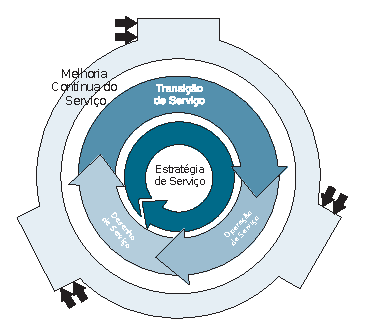
\includegraphics[width=.70\textwidth]{figuras/ciclo_itil.eps} 
  \caption{Ciclo de Vida de Serviços \acrshort{itil} v3 (Adaptada de \cite{servicestrategy}).}
  \label{fig-ciclo-de-vida-itil} 
\end{figure}

Cada fase deste ciclo é documentado através da produção de um livro, e cada um destes tem como objetivo fornecer um conjunto de boas práticas para uma das fases de implantação do \acrshort{itil} na organização \cite{servicestrategy, introductoryoverviewofitil, arraj2010itil}. Deve-se salientar que um princípio chave de cada uma das etapas do ciclo de vida de serviços é a entrega dos valores necessários para que seja possível o alcance dos objetivos de negócio da organização \cite{commerce2007official}.

\subsection*{Estratégia de Serviço (\textit{Service Strategy})}

\noindent A principal etapa do ciclo de vida de serviços é a Estratégia de Serviço, pois tem como característica o foco na entrega de valores necessários para o atendimento das necessidades do cliente e não apenas na entrega do produto \cite{introductoryoverviewofitil}. A Estratégia de Serviço pode ser definida como um conjunto de orientações de como projetar, desenvolver e implementar o gerenciamento de serviços sobre uma perspectiva de ativo estratégico \cite{itilimplementationfailure}. Seu objetivo está na definição da perspectiva, posição, planos e padrões que são necessários para que o prestador de serviço seja capaz de executar e atender os resultados que são esperados pela organização \cite{servicestrategy}.

Outra característica da Estratégia de Serviço está no fornecimento de orientação aos prestadores de serviços sobre a forma como os processos e as políticas de gerenciamento devem ser planejados, desenvolvidos e implantados ao decorrer do ciclo de vida dos serviços \cite{abreu2012implantando}. A execução da fase de Estratégia de Serviço promove as seguintes mudanças na organização \cite{servicestrategy}:

\begin{itemize}
    \item Um entendimento sobre o que é estratégia;
    \item Uma clara identificação e definição dos serviços que os clientes necessitam;
    \item A habilidade de definir como o valor é criado e distribuído;
    \item Identificar oportunidades para explorar e fornecer serviços;
    \item Um modelo claro de prestação de serviço que articula a forma como os serviços serão entregues e com qual propósito; e
    \item Processos que definem a estratégia da organização, quais serviços vão seguir a estratégia, em qual nível de demanda e os meios para garantir a existência de uma relação de trabalho entre o cliente e o provedor de serviços.
\end{itemize}

A Estratégia de Serviço é formada por três principais processos, sendo eles: Gerenciamento Financeiro de \acrshort{ti}, Gerenciamento do Portfólio de Serviços e Gerenciamento da Demanda \cite{abreu2012implantando}.

A etapa de gerenciamento financeiro consiste na gerência da parte de finanças do Portfólio de Serviços de \acrshort{ti} da organização de forma a oferecer o equilíbrio econômico necessário na execução dos serviços \cite{abreu2012implantando}. O processo de gerência financeira, por sua vez, tem como finalidade fornecer um nível adequado de recursos financeiros necessários para projetar, desenvolver e fornecer serviços de \acrshort{ti} que atendam às necessidades da organização \cite{introductoryoverviewofitil}. Uma gestão financeira rigorosa proporciona uma maior visibilidade operacional, percepção e tomada de decisões superiores para as organizações de \acrshort{ti} de forma a oferecer aos negócios da organização uma melhor percepção sobre o real valor dos serviços prestados\cite{commerce2007official}.

O Gerenciamento de Portfólio tem como objetivo garantir ao prestador de serviços de \acrshort{ti} uma combinação correta de serviços de forma a equilibrar os investimentos em \acrshort{ti} com a capacidade de atender os resultados de negócio \cite{introductoryoverviewofitil}. A etapa referente à gerência de portfólio visa, sobretudo, governar os investimentos da empresa na gerência de serviços adicionando valor ao negócio e estabelecendo duas categorias de serviços: os serviços de negócios e os serviços de \acrshort{ti} \cite{abreu2012implantando}.

No Gerenciamento de Demanda procura-se gerenciar de maneira síncrona os ciclos de produção de serviços e os ciclos de consumo dos serviços \cite{abreu2012implantando}. Esse processo é um aspecto crítico do gerenciamento de serviços, pois em casos de má administração das demandas é criado um sentimento de incerteza sobre a execução do serviço que se transforma em um grande fator de risco aos negócios da organização \cite{introductoryoverviewofitil}.

A Figura \ref{relacao-etapas-itil} apresenta a relação entre as etapas do ciclo de vida de serviços do \acrshort{itil}, na qual podemos constatar que a Estratégia de Serviço é o centro  do ciclo de vida de serviços, pois representa a principal fonte de requisitos para as demais etapas, já a Melhoria Contínua do Serviço está presente em todos os estágios por fornecer suporte às demais etapas através de medições e avaliações de desempenho sobre cada uma das etapas do ciclo de vida de serviços \cite{abreu2012implantando}.

\begin{figure}[!ht]
  \centering
  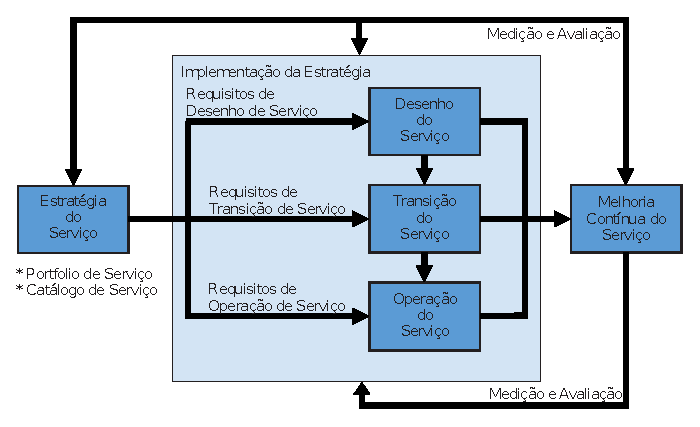
\includegraphics[width=.70\textwidth]{figuras/relacao-etapas-itil.eps} 
  \caption{Relação entre as etapas do Ciclo de Vida de Serviços (Adaptada de \cite{abreu2012implantando, servicestrategy}).}
  \label{relacao-etapas-itil} 
\end{figure}

\subsection*{Desenho de Serviço (\textit{Service Design})}

\noindent O Desenho de Serviço é um conjunto de orientações que objetiva a concepção e o desenvolvimento de serviços e gerenciamento de processos, com foco na concepção do serviço de \acrshort{ti} por meio de práticas de Governança de \acrshort{ti}, processos e políticas que têm como principal objetivo satisfazer as necessidades do cliente. Essa prática resulta em uma entrega de serviços com qualidade e um menor preço de produção \cite{itilimplementationfailure, servicedesign}.

Através dessa etapa é apresentada uma série de orientações sobre o planejamento e desenvolvimento do gerenciamento de serviços e processos almejando promover melhorias na entrega de valor aos clientes no decorrer do ciclo de serviços, além de fornecer um aspecto detalhado do gerenciamento do catálogo de serviços, de sua capacidade, continuidade, da segurança da informação, dentre outros \cite{abreu2012implantando}.

\noindent São objetivos do Desenho de Serviço \cite{servicedesign}:

\begin{itemize}
    \item Possibilitar com mais precisão a estimativa de custos, tempo, exigência e riscos associados com os recursos relacionados com a etapa de planejamento de serviços;
    \item Facilitar a criação de métodos de planejamento com facilidade tornando mais fácil de serem seguidas;
    \item Reduzir os atrasos causados pela necessidade de replanejamento dos serviços antes da conclusão da Transição de Serviço.
    \item Proporcionar melhoria no gerenciamento das expectativas das partes interessadas que inclui clientes, usuários, fornecedores, parceiros do projeto;
    \item Aumentar a confiança na entrega de serviços novos ou modificados; e
    \item Certificar que a criação de serviços novos ou modificados tenham fácil manutenção e baixo custo.
\end{itemize}

A etapa de Desenho de Serviço é composto por sete principais processos, são eles: Gerenciamento do Catálogo de Serviços, Gerenciamento do Nível de Serviço, Gerenciamento da Capacidade, Gerenciamento da Disponibilidade, Gerenciamento da Continuidade do Serviço, Gerenciamento da Segurança da Informação e Gerenciamento de Fornecedores \cite{abreu2012implantando}. A Figura \ref{relacao-desenho-servico} mostra uma visão geral dos processos da etapa de Desenho de Serviço, evidenciando a maneira como é feita a interligação entre os processos \cite{abreu2012implantando}.

O catálogo de serviços consiste em um banco de dados ou documento que estrutura todas as informações sobre os serviços de \acrshort{ti}, o que inclui informações sobre as entregas, preços, pontos de contatos e ordenação dos processos de solicitação dos serviços \cite{servicedesign}.

O Gerenciamento do Catálogo de Serviços fornece uma fonte central com informações sobre os serviços entregues pela organização prestadora de serviços de \acrshort{ti}, disponibilizando uma visão mais precisa e detalhada sobre quais são os serviços disponíveis oferecidos pela \acrshort{ti} \cite{introductoryoverviewofitil}. O Catálogo de Serviços tem duas subdivisões \cite{abreu2012implantando}:

\begin{itemize}
    \item Catálogo de Serviços de Negócio: engloba a visão do cliente sobre os serviços de \acrshort{ti}, além de proporcionar um melhor relacionamento deste com os processos e estruturas organizacionais do negócio; e
    \item Catálogo de Serviços Técnicos: oferece maiores detalhes técnicos de todos os serviços oferecidos ao cliente, detalhando como é o relacionamento do cliente com os serviços de suporte, itens de configurações e demais pormenores que são necessários para a execução do serviço prestado.
\end{itemize}

\begin{figure}[!h]
  \centering
  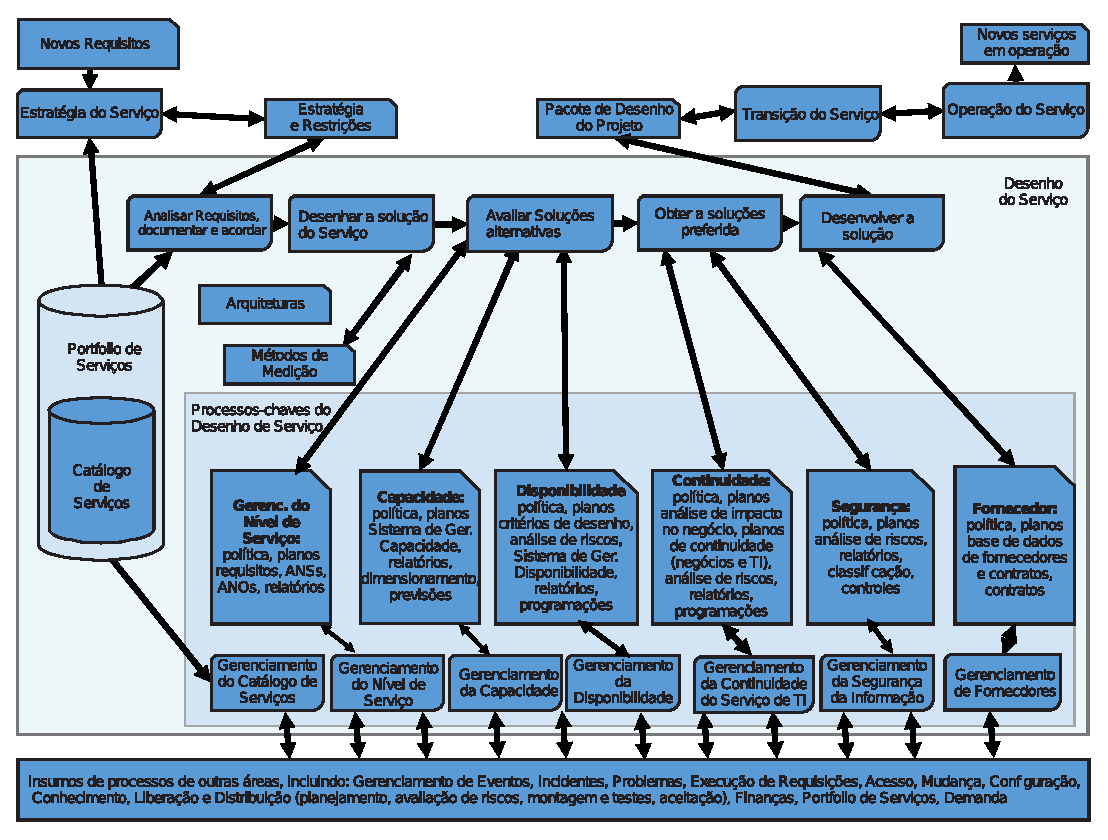
\includegraphics[width=1\textwidth]{figuras/desenho-servico.eps} 
  \caption{Visão geral dos processos do Desenho de Serviço (Adaptada de \cite{abreu2012implantando, servicedesign}).}
  \label{relacao-desenho-servico} 
\end{figure}

Outro item definido pelo Desenho de Serviço é o processo de \gls{slm_itil}, o \acrshort{slm_itil} é um documento utilizado pelos prestadores de serviços de \acrshort{ti} e clientes que visa proporcionar melhorias na qualidade dos serviços prestados pela \acrshort{ti} \cite{introductoryoverviewofitil}. Sua utilização tem como propósito a definição de um ciclo contínuo de atividades que envolvem o planejamento, coordenação, elaboração e estabelecimento de acordo e metas de desempenho através de um acordo de responsabilidade mútua entre os envolvidos \cite{abreu2012implantando}.

É papel do \acrshort{slm_itil} negociar, concordar e documentar as metas dos serviços de \acrshort{ti} verificando se estão adequadas com os negócios e com o \acrshort{sla}, sendo possível em sequência, iniciar a fase de monitoramento e produção de relatórios sobre as entregas dos serviços prestados \cite{introductoryoverviewofitil}. 

Desta maneira, observa-se que seu principal propósito é assegurar que todas as operações de serviços e seus desempenhos sejam medidos de forma consistente e profissional por toda a organização de \acrshort{ti}, de modo que os relatórios emitidos durante a execução dos serviços tenham como foco atender as necessidades de negócio do cliente \cite{introductoryoverviewofitil}.

É definido no processo de Gerenciamento da Capacidade questões que asseguram a capacidade da infraestrutura de \acrshort{ti} de absorver a crescente demanda de novos negócios requisitados pela organização, de forma que minimize os riscos e interrupções que possam ocorrer pelos prestadores de serviços da \acrshort{ti} \cite{abreu2012implantando}.

O fator de sucesso do processo em questão está na sua utilização durante a fase de planejamento de serviço, uma vez que o seu principal objetivo está na capacidade de fornecer um foco maior na gestão de problemas relacionados ao desempenho do tempo de resposta da \acrshort{ti} em atender as demandas de negócio da organização \cite{introductoryoverviewofitil}.

Um dos principais objetivos do Gerenciamento da Disponibilidade está em promover melhorias na disponibilidade dos serviços fornecidos pela \acrshort{ti}, de forma que as questões relacionadas a disponibilidade do serviço assegurem que os objetivos da organização sejam alcançados de forma custo efetiva \cite{introductoryoverviewofitil}. A preservação do nível de confiabilidade dos serviços de \acrshort{ti} é um fator crítico para que haja confiança sobre a disponibilidade dos serviços oferecidos pela \acrshort{ti}, uma boa execução do processo de gerenciamento de disponibilidade assegura que os riscos de interrupções dos serviços sejam minimizados através da utilização de abordagens de monitoramento das atividades físicas e de solução de incidentes que visam a melhoria contínua da organização de suporte \cite{abreu2012implantando}.

O Gerenciamento da Continuidade do Serviço por sua vez, visa assegurar que os serviços de \acrshort{ti} tenham os recursos necessários para sua continuação, como recursos de infraestrutura, manutenibilidade de serviços e o suporte técnico, e que estes estejam disponíveis sempre que houver necessidade de sua utilização. Isto sugere a existência de um tempo preestabelecido de resposta ao atendimento \cite{abreu2012implantando}.

Assim, o objetivo principal do gerenciamento de continuidade é manter a capacidade de recuperação dos serviços de \acrshort{ti} em corresponder as necessidades definidas na etapa de desenho dos serviços, tendo sempre como meta o cumprimento dos requisitos estabelecidos dentro dos prazos definidos \cite{introductoryoverviewofitil}.

É através do processo de Gerenciamento da Segurança da Informação que são definidos os processos relacionados a garantia da segurança das informações das organizações, utilizadas pelos serviços prestados pela \acrshort{ti}, assegurando a aplicação de políticas de segurança nos serviços de \textit{software} e de \textit{hardware} oferecidos pelos prestadores de serviços em todo o ciclo de vida dos serviços \cite{abreu2012implantando}. Sua proposta é alinhar a segurança da \acrshort{ti} com os negócios da organização, de forma que garanta que as políticas de segurança da informação sejam efetivamente aplicadas, são elas \cite{introductoryoverviewofitil}:

\begin{itemize}
    \item Garantia da disponibilidade e usabilidade da informação quando requisitada;
    \item Garantia da confidencialidade e integridade das informações através de uma política de níveis de permissões de leitura e escrita; e
    \item Garantia de uma transação confiável das informação comerciais.
\end{itemize}

No processo de Gerenciamento de Fornecedores são definidas formas que garantam que os provedores de serviços de \acrshort{ti} atendam às expectativas de negócio da organização, tendo como objetivo assegurar que os serviços sejam executados e atinjam as metas preestabelecidas nos contratos e acordos \cite{introductoryoverviewofitil}. Seu foco está em gerir fornecedores e contratos de forma que seja suprida as necessidades da organização, promovendo melhorias na transparência dos negócios desta e no retorno do valor investido \cite{abreu2012implantando}.

\subsection*{Transição de Serviço (\textit{Service Transition})}

\noindent O objetivo da fase de Transição de Serviço é garantir que serviços novos, modificados ou aposentados atendam às expectativas de negócios que estão documentadas na Estratégia de Serviço e Desenho de Serviço, fornecendo um conjunto de orientações para que ocorram melhorias e aperfeiçoamento das habilidades do prestador de serviços sobre como fazer transição e mudanças de seus serviços durante sua execução no ciclo de vida do \acrshort{itil} \cite{servicetransiction, itilimplementationfailure}. São objetivos da Transição de Serviço \cite{servicetransiction}:

\begin{itemize}
    \item Planejar e gerenciar alterações de serviços de forma eficiente e eficaz;
    \item Gerenciar riscos relacionados a serviços novos, alterados ou aposentados;
    \item Implantar com êxito novas versões dos serviços em ambientes suportados;
    \item Definir expectativas sobre o desempenho do uso de serviços novos ou alterados;
    \item Verificar se as alterações de serviços criam realmente o valor esperado para o negócio; e
    \item Fornecer informações sobre a qualidade dos serviços e bens de serviços.
\end{itemize}

A fase de Transição de Serviço é divido em seis principais processos, são eles: Gerenciamento de Mudanças, Gerenciamento de Ativos de Serviço e da Configuração, Gerenciamento da Liberação e Distribuição, Validação e Teste do Serviço, Avaliação e Gerenciamento do Conhecimento \cite{abreu2012implantando, servicetransiction}.

O processo de Gerenciamento de Mudanças visa minimizar o impacto causado pelas transformações provocadas durante a execução dos serviços, ela busca assegurar um tratamento sistemático e padronizado das possíveis mudanças que possam ocorrer no ambiente operacional da organização \cite{abreu2012implantando}. A gestão de mudanças tem como foco proporcionar um melhor controle em todo o ciclo de vida de serviços permitindo que sejam feitas alterações benéficas com um efeito mínimo de perturbação sobre a execução dos serviços prestados pela \acrshort{ti} \cite{introductoryoverviewofitil}.

O Gerenciamento de Ativos de Serviço e da Configuração é responsável por fazer a identificação dos registros e controle de verificação de ativos de itens de serviços de configuração, como componentes de \acrshort{ti}, itens de \textit{hardware}, \textit{software} e documentação associada aos serviços fornecidos pela \acrshort{ti} \cite{abreu2012implantando}. O processo procura fornecer apoio aos negócios fornecendo informações necessárias para gerenciar os demais serviços da etapa de ciclo de vida do \acrshort{itil}, o que contribui o sucesso em todas as etapas do ciclo de gerenciamento de serviços, proporcionando uma obtenção do máximo valor dos ativos de serviços \cite{introductoryoverviewofitil}.

O desenvolvimento do Gerenciamento da Liberação e Distribuição está centrado na gerência de um conjunto de mudanças sobre um serviço de \acrshort{ti}, sendo estas devidamente autorizadas, por exemplo, atividades de planejamento e configuração de itens de \textit{software} e \textit{hardware}, com o propósito de criar um conjunto de componentes finais para serem implantados em blocos no ambiente de produção \cite{abreu2012implantando}. Desse modo, seu propósito consiste em fornecer formas de planejamento da implantação dos serviços, assim como estratégias para programar o lançamento de novas funcionalidades de forma que novas modificações feitas não afetem o funcionamento de serviços já em produção \cite{introductoryoverviewofitil}.

A etapa de Validação e Teste do Serviço está relacionada com a garantia da qualidade de entrega de um serviço novo ou alterado, sendo feito testes para a validação do mesmo com o objetivo de garantir que seja entregue um serviço de acordo com o propósito definido na etapa de Desenho do mesmo \cite{abreu2012implantando}. Essa prática propicia a adequação dos serviços às especificações e necessidades de negócio, possibilitando uma maior confiança no lançamento de novas atividade e garantindo a entrega de valor ao cliente \cite{introductoryoverviewofitil}.

O processo de Avaliação é responsável pela criação de formas padronizadas para  avaliar o desempenho que uma mudança pode proporcionar nos serviços já em execução mantidas pela \acrshort{ti} em confronto com as metas estipuladas, registrando e gerenciando os desvios encontrados \cite{abreu2012implantando}. O principal resultado obtido, dessa maneira, está na capacidade de geração de relatórios analíticos aos prestadores de serviços de \acrshort{ti} que auxiliarão a equipe responsável a obter uma visão geral sobre quais são as possíveis mudanças a serem realizadas nos processos do \acrshort{itil} para que ocorra uma melhoria na entrega de seus serviços \cite{introductoryoverviewofitil}.

O gerenciamento do conhecimento procura certificar que as informações corretas sejam entregues de forma apropriada para uma pessoa que tenha habilidades para atuar na atividade no tempo esperado, além de informar um conjunto de conhecimentos tais como a experiência de equipe, requisitos, habilidades, as expectativas dos fornecedores e parceiros e histórico de informações \cite{abreu2012implantando}. Sua principal proposta é gerir o conhecimento de forma a partilhar perspectivas, ideias, experiências e informações \cite{introductoryoverviewofitil}

\subsection*{Operação de Serviço (\textit{Service Operation})}

\noindent Operação de Serviço inclui orientações para a obtenção de eficácia na entrega e suporte de serviços de forma a assegurar o valor da entrega do serviço ao cliente. Esta fase configura-se como uma das mais críticas do ciclo de vida de serviços do \acrshort{itil}, pois mesmo que tenha um bom planejamento e implementação dos processo, todo o trabalho será nulo caso a organização não tenha uma cultura de monitoramento de informações como desempenho, avaliação de métricas e a coleta de dados operacionais \cite{serviceoperation, itilimplementationfailure}. São objetivos da etapa de Operação de Serviço \cite{serviceoperation}:

\begin{itemize}
    \item Manter a satisfação e confiança nos negócios da \acrshort{ti} através da entrega eficaz e eficiente dos serviços, além de fornecer suporte a eles;
    \item Minimizar o impacto de interrupções de serviços em atividades do dia-a-dia; e
    \item Certificar que os serviços de \acrshort{ti} sejam prestados apenas a setores autorizados.
\end{itemize}

A etapa de Operação de Serviço é dividida em um conjunto de cinco processos, são eles: Gerenciamento de Eventos, Gerenciamento de Incidentes, Execução de Requisições, Gerenciamento de Problemas e Gerenciamento do Acesso \cite{serviceoperation, abreu2012implantando}. A Figura \ref{relacao-processos-service-operation} apresenta os processos envolvidos na etapa de operação de serviço \cite{abreu2012implantando}.

\begin{figure}[!h]
  \centering
  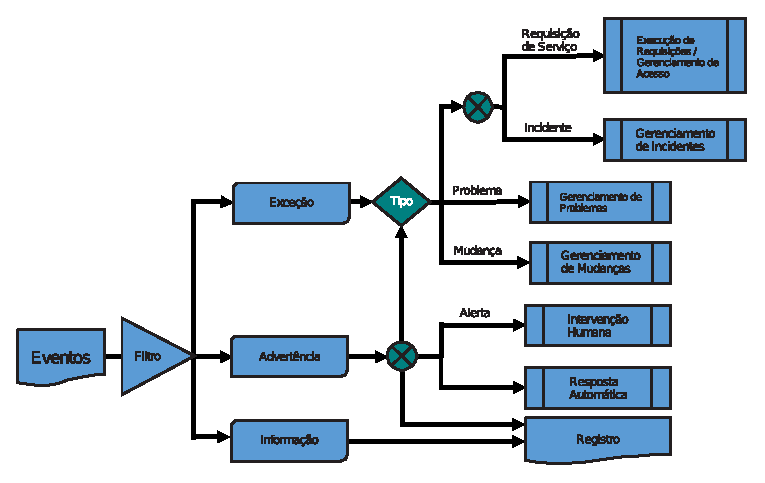
\includegraphics[width=.80\textwidth]{figuras/processos-service-operation.eps} 
  \caption{Visão geral dos processos do Operação de Serviço (Adaptada de \cite{abreu2012implantando, serviceoperation}).}
  \label{relacao-processos-service-operation} 
\end{figure}

O Gerenciamento de Eventos propõe a promoção de uma monitoria de todos os eventos que ocorrem na infraestrutura da \acrshort{ti}, tendo como intuito proporcionar a normalidade das operações do serviço \cite{abreu2012implantando}. Um evento pode indicar que algo não está funcionando corretamente, e nesse passo é necessária a criação de uma política de monitoramento de processos com o objetivo de apontar quais atividades estão dentro da normalidade e identificar que estejam atrapalhando o funcionamento normal de um determinado conjunto de serviços \cite{introductoryoverviewofitil}. 

Através do processo de gerenciamento de eventos busca-se promover melhorias no seu gerenciamento durante a execução no ciclo de vida de serviços, concentrando-se na geração e detecção de notificações significativas sobre eventuais problemas \cite{introductoryoverviewofitil}.

No Gerenciamento de Incidentes espera-se alcançar uma restauração da normalidade da operação de um serviço em um menor tempo possível, minimizando os impactos gerados nos negócios devido a ocorrência de eventuais incidentes, e focando na entrega de valor aos clientes dentro dos padrões acordados \cite{abreu2012implantando}. No entanto, incidentes são frequentemente detectados e reportados por meio da utilização de ferramentas de monitoramento ou através da reclamação feita diretamente na central de atendimento. Após feito o levantamento dos incidentes eles são catalogados e ordenados de acordo com sua prioridade e direcionados de acordo a sua necessidade de correção ao setor responsável. \cite{introductoryoverviewofitil}.

A Execução de Requisições define a forma como devem ser tratadas as requisições realizadas pelos usuários dos serviços de \acrshort{ti}, sendo elas originadas
de uma solicitação de serviço ou de uma simples solicitação de informação\cite{abreu2012implantando}.

A principal finalidade do processo de execução de requisições está em permitir que usuários tenham acesso às informações sobre os serviços prestados criando um canal de comunicação que torna possível fazer elogios ou reclamações sobre eventuais problemas com os serviços fornecidos pela \acrshort{ti} \cite{introductoryoverviewofitil}.

O método referente ao Gerenciamento de Problemas tem como propósito minimizar os impactos adversos que os incidentes causam para os negócios, de forma a proporcionar melhorias nas estratégias adotadas para a prevenção de incidentes \cite{abreu2012implantando}. As adversidades detectadas são classificadas de maneira semelhante ao gerenciamento de incidentes, tendo como característica principal a busca das causas do problema \cite{introductoryoverviewofitil}. Para solução deste é feito um levantamento de propostas contendo soluções alternativas \cite{introductoryoverviewofitil, serviceoperation}.

O Gerenciamento do Acesso, como o nome sugere, é responsável pelo controle de acesso do usuário, restringindo através de autorizações a possibilidade de alcance a informações e serviços, o que torna o processo mais seguro \cite{abreu2012implantando}.

O processo de Gerenciamento do Acesso visa ajudar o gerenciamento da confidencialidade, disponibilidade, integridade dos dados e propriedade intelectual das informações presentes no sistema \cite{introductoryoverviewofitil}. Ele inclui a verificação da identidade do usuário e suas restrições de acesso aos serviços, além de garantir que mudanças de permissões sejam feitas caso haja a necessidade \cite{introductoryoverviewofitil}.

\subsection*{Melhoria Contínua do Serviço (\textit{Continual Service Improvement})}

\noindent Um dos principais objetivos da Melhoria Contínua do Serviço está no alinhamento dos serviços de \acrshort{ti} com as necessidades de negócio da organização através da identificação e implementação de aperfeiçoamentos nos serviços prestados pela \acrshort{ti}. Tais mudanças são feitas através de uma melhor abordagem do ciclo de vida a fim de apoiar as demais etapas do mesmo, como a Estratégia de Serviço, Desenho de Serviço, Transição de Serviço e Operação de Serviço \cite{continualserviceimprovement}.

A Melhoria Contínua do Serviço serve como um guia que contém orientações de como criar e manter valor para o cliente através de um conjunto de melhorias no planejamento e na introdução de novos serviços, combinando princípios, práticas e métodos de aperfeiçoamento da qualidade da gestão dos serviços de \acrshort{ti} \cite{itilimplementationfailure}. São objetivos do Melhoria Contínua do Serviço \cite{continualserviceimprovement}:

\begin{itemize}
    \item Revisar, analisar além de fazer recomendações de mudanças para melhorias nos processos do ciclo de vida como o Estratégia de Serviço, Desenho de Serviço, Transição de Serviço, Operação de Serviço e até mesmo da própria Melhoria Contínua do Serviço;
    \item Revisar e analisar o nível de realização do serviço;
    \item Identificar e implementar atividades específicas com o objetivo de melhorar a qualidade dos serviços de \acrshort{ti}; e
    \item Melhorar a eficácia do custo de entrega dos serviços de \acrshort{ti} sem que seja necessário sacrificar a satisfação do cliente.
\end{itemize}

A Figura \ref{relacao-processos-csi} mostra os conceitos envolvidos no estágio de Melhoria Contínua do Serviço cuja base é composta por dois principais processos, sendo eles o Relato do Serviço e Medição do Serviço.

\begin{figure}[!h]
  \centering
  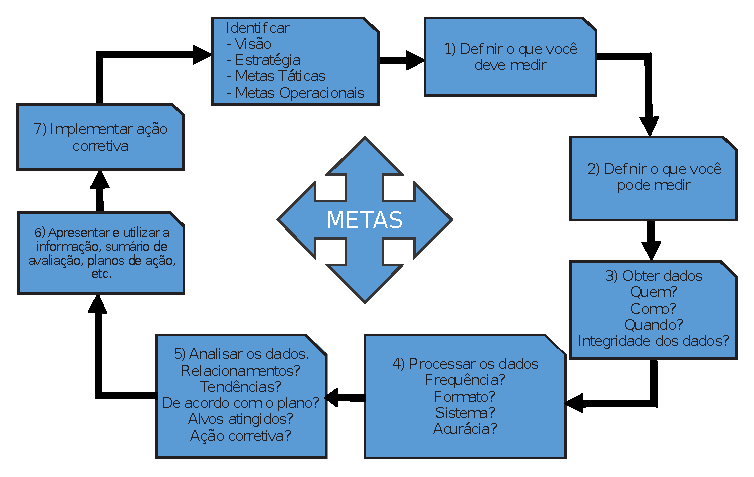
\includegraphics[width=.70\textwidth]{figuras/processos-ci.eps} 
  \caption{Visão geral dos processos do Melhoria Contínua do Serviço (Adaptada de \cite{abreu2012implantando, continualserviceimprovement}).}
  \label{relacao-processos-csi} 
\end{figure}

O processo de Relato do Serviço é a formalização de um conjunto de relatórios que contém informações coletadas a partir do monitoramento das estregas de serviços, a identificação de dados como definição do objetivo do serviço relatado e do público-alvo \cite{abreu2012implantando}.

A utilização de um relatório contendo apenas a adesão ou não da \acrshort{sla} não é autossuficiente, assim, é de grande importância que os prestadores de serviços de \acrshort{ti} possam criar uma abordagem acionável para a elaboração dos relatórios de serviços, sendo necessário que contenha informações que responda as seguintes perguntas \cite{introductoryoverviewofitil}: 

\begin{itemize}
    \item Porque aconteceu determinados eventos?
    \item Quem realizou tal ação?
    \item Como garantir que antigos incidentes não impactem novamente o serviço?
    \item Como melhorar a prestação de serviço?
\end{itemize}

A Medição do Serviço foca no fornecimento de uma visão completa e orientada sobre a integração dos serviços aos valores de negócios da organização. Para que haja tal modelo de medição é necessário que sejam estabelecidos diferentes níveis de avaliações para sua apreciação através dos relatórios \cite{abreu2012implantando}. Existem três tipos de métricas que uma organização necessita para recolher e apoiar as atividades da etapa de Melhoria Contínua do Serviço, são elas \cite{introductoryoverviewofitil}: 

\begin{itemize}
    \item Métricas de Tecnologia, que em muitos casos está diretamente associada a métricas de componentes e base de aplicações, tais como desempenho e disponibilidade;
    \item Métricas de Processo que está diretamente ligada aos indicadores chave de desempenho e métricas de atividade; e
    \item Métricas de Serviços que demostram resultados de serviços fim-a-fim, onde métricas de componentes e tecnologia são utilizadas para calcular as métricas de serviço.
\end{itemize}

\section{Especificação de Requisito de \textit{Software}}

\noindent É um grande desafio para os desenvolvedor o ato de saber analisar e projetar \textit{software} de forma a satisfazer os requisitos que os clientes esperam encontrar no produto \cite{pressmanengenharia}. Assim, um bom planejamento e definição dos requisitos para a construção do \textit{software} proporciona um melhor entendimento do projeto, fornecendo aos desenvolvedores e clientes um documento claro com informações a respeito dos requisitos necessários para o desenvolvimento do produto especificado \cite{pressmanengenharia}. 
Especificações como a \gls{ieee} 830 \cite{ieee1998ieee} fornecem um conjunto de informações contendo descrições importantes para o desenvolvimento do \textit{software} em questão, como levantamento de Requisitos Funcionais, Requisitos não Funcionais além de uma descrição detalhada do serviço projetado.

A documentação \acrshort{ieee} 830/98 é definida pela \acrshort{ieee} \textit{Standards}, onde são descritas informações com as melhores práticas para especificação de \textit{software} \cite{ieee1998ieee}.  Sua finalidade está em fornecer diversos atributos que são necessários para o desenvolvimento e implantação de serviços de \textit{software}. O uso do \gls{srs} tem como principal benefícios \cite{ieee1998ieee}:

\begin{itemize}
    \item Estabelecer bases de acordo entre os clientes com os fornecedores do serviço de forma a definir o que \textit{software} deve fazer;
    \item Promover uma redução do esforço para desenvolvimento do projeto, pois a \acrshort{srs} define todos os requisitos necessários para o desenvolvimento e implantação do \textit{software}; e
    \item Proporcionar uma melhoria na estimativa de entrega das atividades e etapas de finalização do \textit{software}.
\end{itemize}

\section{Metodologia de Desenvolvimento Ágil}

\noindent A adoção de métodos ágeis de desenvolvimento de \textit{software} tem sido utilizada por diversas empresas de desenvolvimento. A adesão de tais práticas visa, sobretudo, tornar o planejamento e execução de projetos mais versáteis e adaptáveis à realidade de mudanças diárias de requisitos de \textit{software} \cite{pressmanengenharia, rubin2012essential}.

\subsection{Manifesto Ágil}

\noindent O termo agilidade surgiu no ano de 2001 por Kent Beck e mais 16 desenvolvedores renomados da área de \textit{software}, dando origem ao termo ``\textit{Agile Alliance}'', culminando na assinatura de um manifesto a favor do desenvolvimento ágil de \textit{software} \cite{pressmanengenharia}. O Manifesto Ágil é um movimento precursor do surgimento dos métodos ágeis de desenvolvimento que tem como princípio a busca por maneiras de implementar um \textit{software} de forma ágil. São princípios fundamentais do manifesto ágil \cite{agilemanifesto}:

\begin{itemize}
    \item \textbf{Indivíduos e interações} mais que processos e ferramentas;
    \item \textbf{\textit{Software} em funcionamento} mais que documentação abrangente;
    \item \textbf{Colaboração com o cliente} mais que negociação de contratos; e
    \item\textbf{Responder a mudanças} mais que seguir um plano.
\end{itemize}

Beck \cite{agilemanifesto} afirma que mesmo que se tenha um maior valor nos itens à direita, os princípios do manifesto ágil focam mais nos itens da esquerda.

\subsection{Metodologia \textit{Scrum}}

\noindent O \textit{Scrum} é uma metodologia de desenvolvimento ágil de \textit{software} criado inicialmente por Jeff Sutherland no início de 1990 \cite{pressmanengenharia}. Uma característica presente nele é o fato de sua ideologia seguir também os princípios presentes no manifesto ágil, tendo como propósito orientar as atividades estruturais de desenvolvimento de \textit{software}, como o levantamento de requisitos, análise dos processos, planejamento do projeto e métodos de evolução e entregas de \textit{software} \cite{pressmanengenharia}.

A Figura \ref{fig-ciclo-scrum} mostra o ciclo de atividades da metodologia \textit{Scrum} de desenvolvimento ágil, onde diversos termos são utilizados para caracterizar as etapas presentes na metodologia, como o \textit{Product Backlog}, \textit{Sprint Backlog}, \textit{Daily Scrum Meeting} e o \textit{Potentially Shippable Product Increment} \cite{pressmanengenharia}.

\begin{figure}[!h]
  \centering
  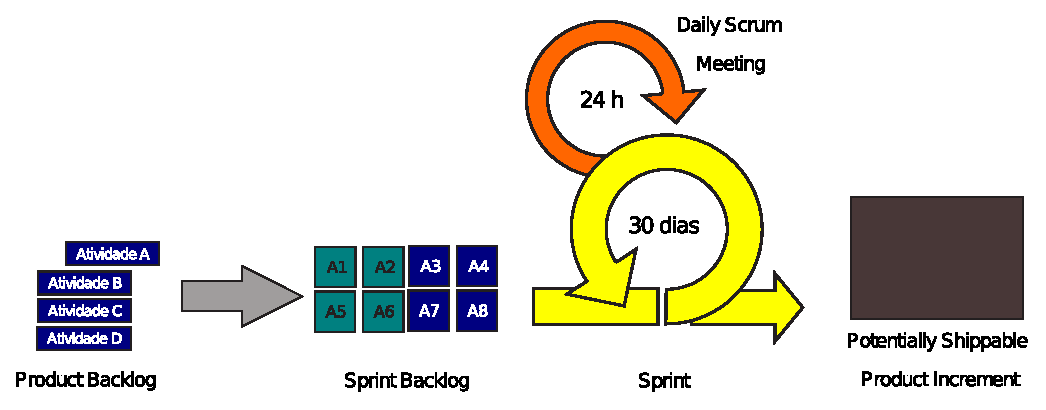
\includegraphics[width=1\textwidth]{figuras/scrum_ciclo.eps} 
  \caption{Ciclo de atividades da metodologia \textit{Scrum} (Adaptada de \cite{pressmanengenharia}).}
  \label{fig-ciclo-scrum} 
\end{figure}

Cada fase presente no ciclo de atividades do \textit{Scrum} tem um papel importante para o seu sucesso na implantação dos serviços de \textit{software}. Sua divisão consiste em \textit{Sprints} que são ciclos de atividades catalogadas pelo \textit{Product Backlog}, sendo dever do \textit{Product Owner} definir quais atividades deverão ser executadas primeiro no projeto através da etapa de \textit{Sprint Planning Meeting} \cite{rubin2012essential}.

O \textit{Scrum} é um aprimoramento da abordagem interativa e incremental para a entrega de \textit{software} orientado a objetos, inicialmente a metodologia foi documentada por Pittman mas posteriormente seus conceitos foram expandidos por Booch \cite{schwaber1997scrum}. De forma geral o \textit{Scrum} é uma metodologia para o gerenciamento de melhorias contínuas na manutenção de um projeto de \textit{software} já existente ou em desenvolvimento \cite{schwaber1997scrum}.

\subsection*{\textit{Product Backlog}}

\noindent Outra característica desta metodologia é a execução da tarefa com maior risco ser feita primeiro, ficando para o \textit{Product Owner} o dever de gerenciar quais tarefas devem ser priorizadas primeiro, influenciando assim todo o andamento da execução das atividades no \textit{Scrum} \cite{rubin2012essential}. A Figura \ref{product-backlog} mostra como é organizada as tarefas em um ordenamento de prioridades de execução (da mais alta prioridade para o de menor prioridade), sendo a definição das prioridades das atividades conhecida como \textit{Product Backlog} \cite{rubin2012essential}.

\begin{figure}[!h]
  \centering
  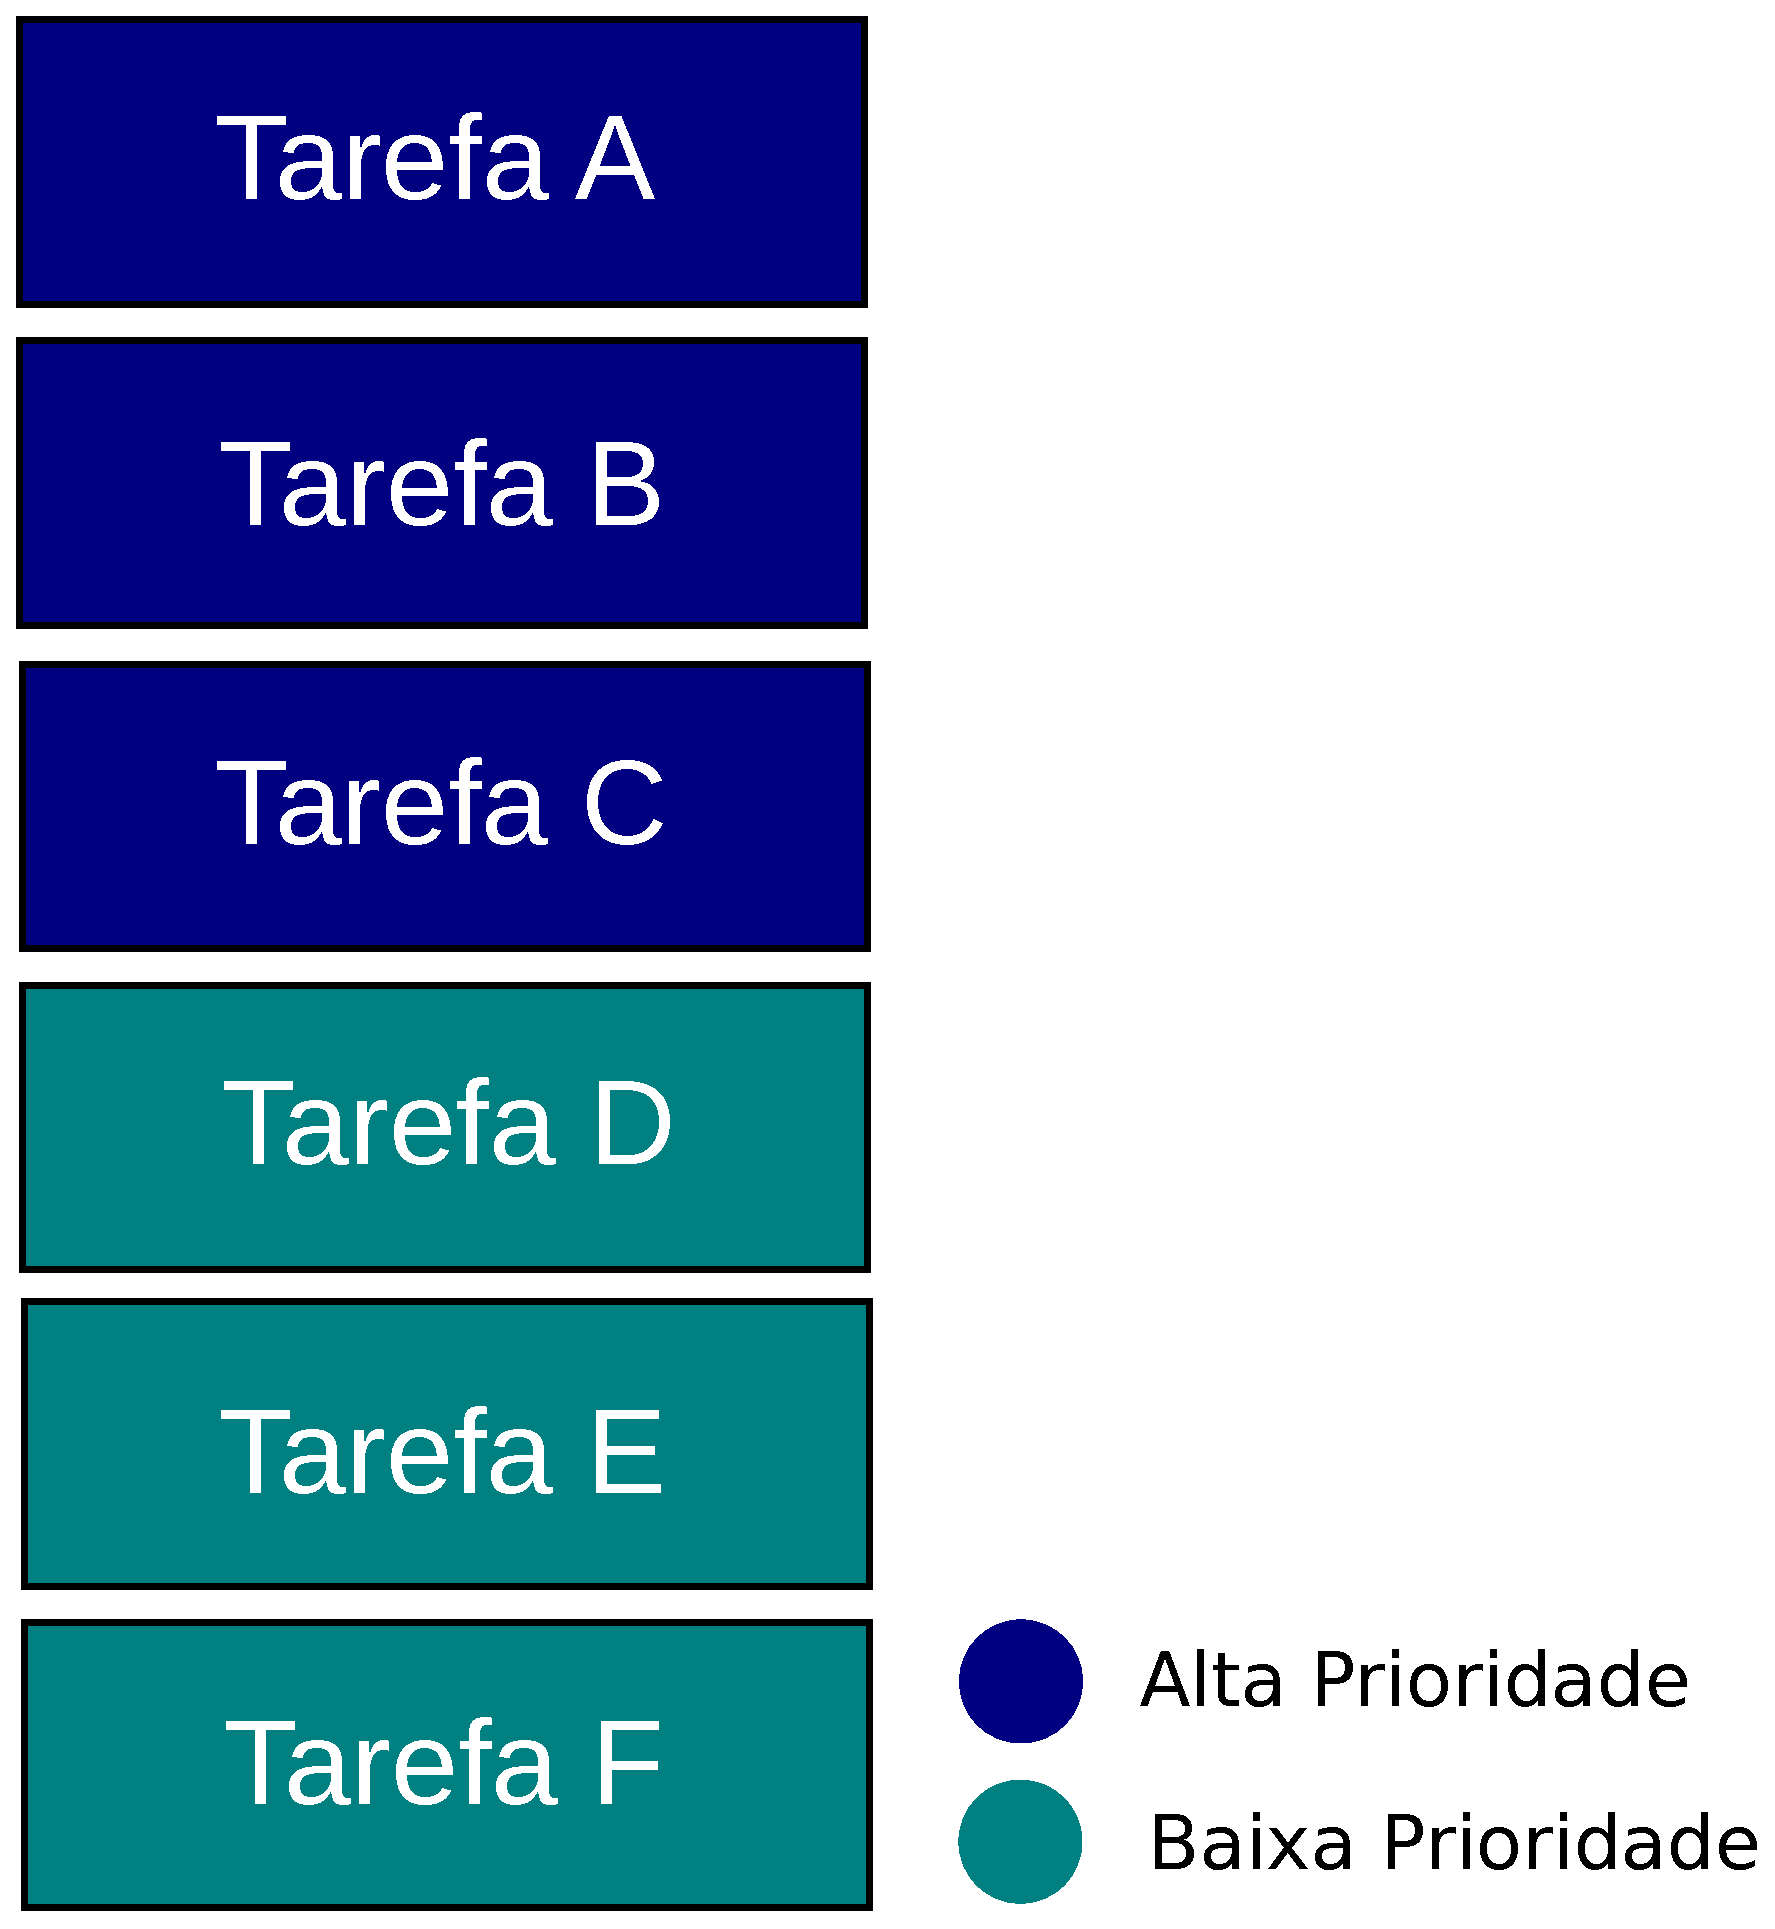
\includegraphics[width=.40\textwidth]{figuras/product_backlog3.eps} 
  \caption{Fase de \textit{Product Backlog} do \textit{Scrum} (Adaptada de \cite{rubin2012essential}).}
  \label{product-backlog} 
\end{figure}

O \textit{Product Backlog} consiste em uma pilha de atividades a serem realizadas pela equipe \textit{Scrum}, em que cada uma de atividade contém seu grau prioridade de execução o que influencia o ordenamento das tarefas a serem executadas \cite{rubin2012essential}.

\subsection*{\textit{Sprint Backlog}}

\noindent O \textit{Sprint Backlog} é uma fase do \textit{Scrum} onde as atividades são catalogadas e priorizadas pelo \textit{Product Backlog} e em sequência são agrupadas em forma de \textit{Sprints} de atividades, que tem como característica um conjunto de atividades prioritárias a serem realizadas pela equipe \textit{Scrum} \cite{pressmanengenharia, rubin2012essential}.

A Figura \ref{sprint-backlog} mostra o processo de definição do \textit{Sprint Backlog}, sendo cada atividade presente no \textit{Product Backlog} subdividida no \textit{Sprint Planning} através da criação de subconjuntos de atividades contendo as tarefas mais importantes definidas inicialmente pelo \textit{Product Owner} \cite{rubin2012essential}.

\begin{figure}[!h]
  \centering
  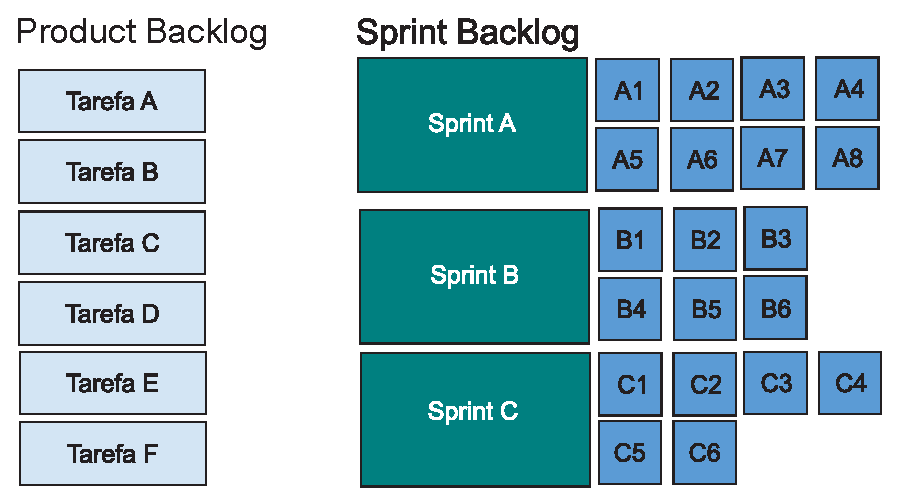
\includegraphics[width=.70\textwidth]{figuras/sprint-backlog.eps} 
  \caption{Fase de criação do \textit{Sprint Backlog} (Adaptada de \cite{rubin2012essential}).}
  \label{sprint-backlog} 
\end{figure}

\subsection*{\textit{Daily Scrum Meeting}}

\noindent O processo do \textit{Daily Scrum Meeting} visa criar reuniões diárias com duração de 15 minutos com os envolvidos no projeto, sendo dever do \textit{Scrum Master} auxiliar o andamento do projeto e organizar as reuniões de forma que seja feita analise do progresso da equipe frente as metas estabelecidas pelo \textit{Sprint} \cite{rubin2012essential}. Uma característica presente nestas reuniões é que os envolvidos permanecem em pé, com a finalidade de tornar as reuniões rápidas e objetivas. A cada reunião todos os membros da equipe respondem diariamente as seguintes perguntas feitas pelo \textit{Scrum Master} \cite{pressmanengenharia}:

\begin{itemize}
    \item O que você realizou desde a última reunião de equipe?
    \item Quais obstáculos está encontrando?
    \item O que você planeja realizar até a próxima reunião da equipe?
\end{itemize}

Outro dever do \textit{Scrum Master} é avaliar cada uma das respostas dadas pelos membros da equipe \textit{Scrum} e procurarventender e planejar novas formas para solucionar os problemas que foram catalogados durante aplicação do questionário \cite{pressmanengenharia, rubin2012essential}.

\subsection*{\textit{Potentially Shippable Product Increment}}

\noindent A fase de \textit{Potentially Shippable Product Increment} é o resultado das execuções das tarefas definidas no \textit{Sprint Planning} que resultaram em um estado de confiança de entrega de novas funcionalidades previstas no \textit{Sprint} \cite{rubin2012essential}.

O conceito de finalização do \textit{Sprint} depende muito dos objetivos que a equipe \textit{Scrum} deseja alcançar. Em alguns casos é decidido pela equipe que seja feito uma entrega parcial das atividades previstas no \textit{Sprint} com o propósito de reunir um conjunto de \textit{feedback} do cliente, que servirá de guia para a equipe contendo informações que os auxiliarão a identificar se as atividades entregues pela equipe estão realmente caminhando em direção ao objetivo desejado \cite{rubin2012essential}.